% Created by tikzDevice version 0.12.6 on 2024-08-04 19:03:11
% !TEX encoding = UTF-8 Unicode
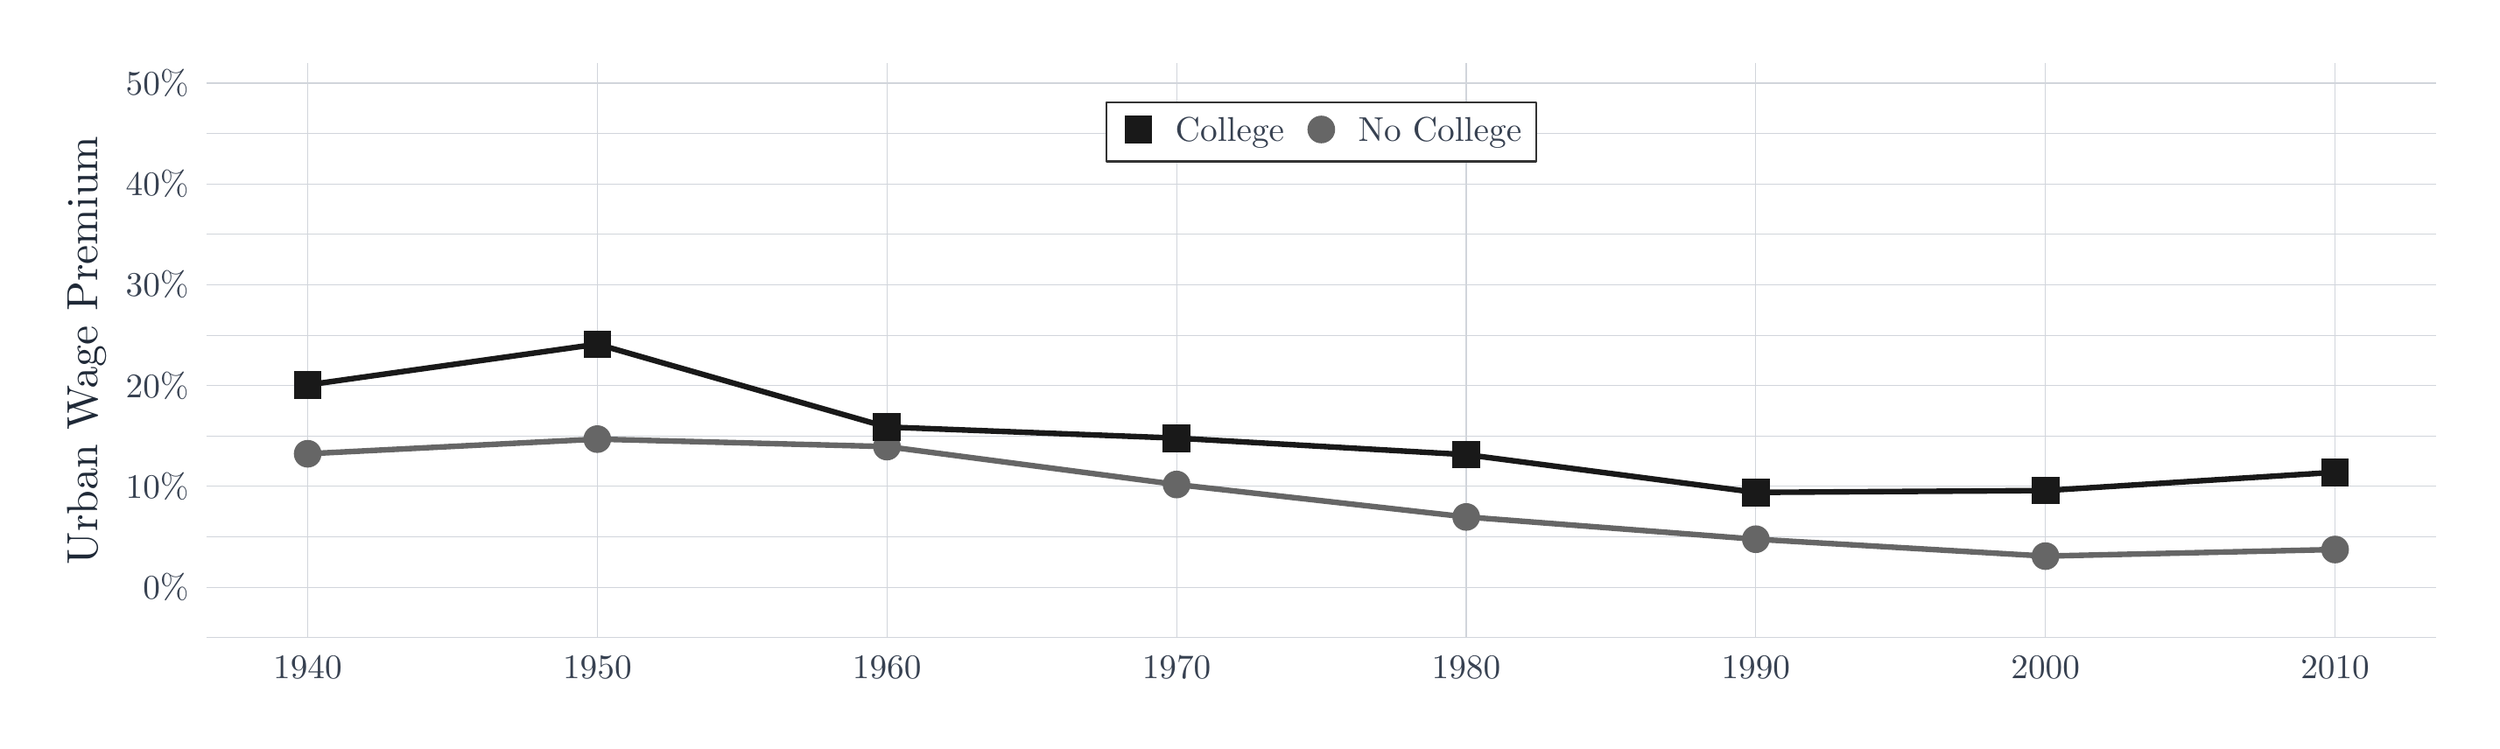
\begin{tikzpicture}[x=1pt,y=1pt]
\definecolor{fillColor}{RGB}{255,255,255}
\path[use as bounding box,fill=fillColor] (0,0) rectangle (1011.78,289.08);
\begin{scope}
\path[clip] (  0.00,  0.00) rectangle (1011.78,289.08);
\definecolor{drawColor}{RGB}{255,255,255}

\path[draw=drawColor,line width= 0.8pt,line join=round,line cap=round,fill=fillColor] (  0.00,  0.00) rectangle (1011.78,289.08);
\end{scope}
\begin{scope}
\path[clip] ( 75.16, 35.76) rectangle (995.78,273.08);
\definecolor{drawColor}{RGB}{255,255,255}
\definecolor{fillColor}{RGB}{255,255,255}

\path[draw=drawColor,line width= 0.8pt,line join=round,line cap=round,fill=fillColor] ( 75.16, 35.76) rectangle (995.78,273.08);
\definecolor{drawColor}{RGB}{209,213,219}

\path[draw=drawColor,line width= 0.4pt,line join=round] ( 75.16, 35.76) --
	(995.78, 35.76);

\path[draw=drawColor,line width= 0.4pt,line join=round] ( 75.16, 77.39) --
	(995.78, 77.39);

\path[draw=drawColor,line width= 0.4pt,line join=round] ( 75.16,119.03) --
	(995.78,119.03);

\path[draw=drawColor,line width= 0.4pt,line join=round] ( 75.16,160.66) --
	(995.78,160.66);

\path[draw=drawColor,line width= 0.4pt,line join=round] ( 75.16,202.30) --
	(995.78,202.30);

\path[draw=drawColor,line width= 0.4pt,line join=round] ( 75.16,243.94) --
	(995.78,243.94);

\path[draw=drawColor,line width= 0.4pt,line join=round] ( 75.16, 56.58) --
	(995.78, 56.58);

\path[draw=drawColor,line width= 0.4pt,line join=round] ( 75.16, 98.21) --
	(995.78, 98.21);

\path[draw=drawColor,line width= 0.4pt,line join=round] ( 75.16,139.85) --
	(995.78,139.85);

\path[draw=drawColor,line width= 0.4pt,line join=round] ( 75.16,181.48) --
	(995.78,181.48);

\path[draw=drawColor,line width= 0.4pt,line join=round] ( 75.16,223.12) --
	(995.78,223.12);

\path[draw=drawColor,line width= 0.4pt,line join=round] ( 75.16,264.75) --
	(995.78,264.75);

\path[draw=drawColor,line width= 0.4pt,line join=round] (117.01, 35.76) --
	(117.01,273.08);

\path[draw=drawColor,line width= 0.4pt,line join=round] (236.57, 35.76) --
	(236.57,273.08);

\path[draw=drawColor,line width= 0.4pt,line join=round] (356.13, 35.76) --
	(356.13,273.08);

\path[draw=drawColor,line width= 0.4pt,line join=round] (475.69, 35.76) --
	(475.69,273.08);

\path[draw=drawColor,line width= 0.4pt,line join=round] (595.25, 35.76) --
	(595.25,273.08);

\path[draw=drawColor,line width= 0.4pt,line join=round] (714.81, 35.76) --
	(714.81,273.08);

\path[draw=drawColor,line width= 0.4pt,line join=round] (834.37, 35.76) --
	(834.37,273.08);

\path[draw=drawColor,line width= 0.4pt,line join=round] (953.93, 35.76) --
	(953.93,273.08);
\definecolor{drawColor}{gray}{0.10}

\path[draw=drawColor,line width= 2.3pt,line join=round] (117.01,140.12) --
	(236.57,156.94) --
	(356.13,122.73) --
	(475.69,118.15) --
	(595.25,111.33) --
	(714.81, 95.73) --
	(834.37, 96.49) --
	(953.93,104.03);
\definecolor{drawColor}{gray}{0.40}

\path[draw=drawColor,line width= 2.3pt,line join=round] (117.01,111.69) --
	(236.57,117.74) --
	(356.13,114.65) --
	(475.69, 98.99) --
	(595.25, 85.60) --
	(714.81, 76.40) --
	(834.37, 69.42) --
	(953.93, 72.14);
\definecolor{fillColor}{gray}{0.40}

\path[fill=fillColor] (117.01,111.69) circle (  5.71);
\definecolor{fillColor}{gray}{0.10}

\path[fill=fillColor] (111.30,134.41) --
	(122.72,134.41) --
	(122.72,145.83) --
	(111.30,145.83) --
	cycle;
\definecolor{fillColor}{gray}{0.40}

\path[fill=fillColor] (236.57,117.74) circle (  5.71);
\definecolor{fillColor}{gray}{0.10}

\path[fill=fillColor] (230.86,151.23) --
	(242.28,151.23) --
	(242.28,162.65) --
	(230.86,162.65) --
	cycle;
\definecolor{fillColor}{gray}{0.40}

\path[fill=fillColor] (356.13,114.65) circle (  5.71);
\definecolor{fillColor}{gray}{0.10}

\path[fill=fillColor] (350.42,117.02) --
	(361.84,117.02) --
	(361.84,128.44) --
	(350.42,128.44) --
	cycle;
\definecolor{fillColor}{gray}{0.40}

\path[fill=fillColor] (475.69, 98.99) circle (  5.71);
\definecolor{fillColor}{gray}{0.10}

\path[fill=fillColor] (469.98,112.44) --
	(481.40,112.44) --
	(481.40,123.86) --
	(469.98,123.86) --
	cycle;
\definecolor{fillColor}{gray}{0.40}

\path[fill=fillColor] (595.25, 85.60) circle (  5.71);
\definecolor{fillColor}{gray}{0.10}

\path[fill=fillColor] (589.54,105.62) --
	(600.96,105.62) --
	(600.96,117.05) --
	(589.54,117.05) --
	cycle;
\definecolor{fillColor}{gray}{0.40}

\path[fill=fillColor] (714.81, 76.40) circle (  5.71);
\definecolor{fillColor}{gray}{0.10}

\path[fill=fillColor] (709.10, 90.02) --
	(720.52, 90.02) --
	(720.52,101.44) --
	(709.10,101.44) --
	cycle;
\definecolor{fillColor}{gray}{0.40}

\path[fill=fillColor] (834.37, 69.42) circle (  5.71);
\definecolor{fillColor}{gray}{0.10}

\path[fill=fillColor] (828.66, 90.78) --
	(840.08, 90.78) --
	(840.08,102.20) --
	(828.66,102.20) --
	cycle;
\definecolor{fillColor}{gray}{0.40}

\path[fill=fillColor] (953.93, 72.14) circle (  5.71);
\definecolor{fillColor}{gray}{0.10}

\path[fill=fillColor] (948.22, 98.32) --
	(959.64, 98.32) --
	(959.64,109.74) --
	(948.22,109.74) --
	cycle;
\end{scope}
\begin{scope}
\path[clip] (  0.00,  0.00) rectangle (1011.78,289.08);
\definecolor{drawColor}{RGB}{55,65,81}

\node[text=drawColor,anchor=base east,inner sep=0pt, outer sep=0pt, scale=  1.42] at ( 67.96, 51.68) {0\%};

\node[text=drawColor,anchor=base east,inner sep=0pt, outer sep=0pt, scale=  1.42] at ( 67.96, 93.31) {10\%};

\node[text=drawColor,anchor=base east,inner sep=0pt, outer sep=0pt, scale=  1.42] at ( 67.96,134.95) {20\%};

\node[text=drawColor,anchor=base east,inner sep=0pt, outer sep=0pt, scale=  1.42] at ( 67.96,176.59) {30\%};

\node[text=drawColor,anchor=base east,inner sep=0pt, outer sep=0pt, scale=  1.42] at ( 67.96,218.22) {40\%};

\node[text=drawColor,anchor=base east,inner sep=0pt, outer sep=0pt, scale=  1.42] at ( 67.96,259.86) {50\%};
\end{scope}
\begin{scope}
\path[clip] (  0.00,  0.00) rectangle (1011.78,289.08);
\definecolor{drawColor}{RGB}{55,65,81}

\node[text=drawColor,anchor=base,inner sep=0pt, outer sep=0pt, scale=  1.42] at (117.01, 18.76) {1940};

\node[text=drawColor,anchor=base,inner sep=0pt, outer sep=0pt, scale=  1.42] at (236.57, 18.76) {1950};

\node[text=drawColor,anchor=base,inner sep=0pt, outer sep=0pt, scale=  1.42] at (356.13, 18.76) {1960};

\node[text=drawColor,anchor=base,inner sep=0pt, outer sep=0pt, scale=  1.42] at (475.69, 18.76) {1970};

\node[text=drawColor,anchor=base,inner sep=0pt, outer sep=0pt, scale=  1.42] at (595.25, 18.76) {1980};

\node[text=drawColor,anchor=base,inner sep=0pt, outer sep=0pt, scale=  1.42] at (714.81, 18.76) {1990};

\node[text=drawColor,anchor=base,inner sep=0pt, outer sep=0pt, scale=  1.42] at (834.37, 18.76) {2000};

\node[text=drawColor,anchor=base,inner sep=0pt, outer sep=0pt, scale=  1.42] at (953.93, 18.76) {2010};
\end{scope}
\begin{scope}
\path[clip] (  0.00,  0.00) rectangle (1011.78,289.08);
\definecolor{drawColor}{RGB}{31,41,55}

\node[text=drawColor,rotate= 90.00,anchor=base,inner sep=0pt, outer sep=0pt, scale=  1.80] at ( 30.15,154.42) {Urban Wage Premium};
\end{scope}
\begin{scope}
\path[clip] (  0.00,  0.00) rectangle (1011.78,289.08);
\definecolor{drawColor}{gray}{0.20}
\definecolor{fillColor}{RGB}{255,255,255}

\path[draw=drawColor,line width= 0.8pt,line join=round,line cap=round,fill=fillColor] (446.74,232.37) rectangle (624.20,256.83);
\end{scope}
\begin{scope}
\path[clip] (  0.00,  0.00) rectangle (1011.78,289.08);
\definecolor{drawColor}{RGB}{255,255,255}
\definecolor{fillColor}{RGB}{255,255,255}

\path[draw=drawColor,line width= 0.8pt,line join=round,line cap=round,fill=fillColor] (452.74,238.37) rectangle (467.20,252.83);
\end{scope}
\begin{scope}
\path[clip] (  0.00,  0.00) rectangle (1011.78,289.08);
\definecolor{fillColor}{gray}{0.10}

\path[fill=fillColor] (454.26,239.89) --
	(465.68,239.89) --
	(465.68,251.31) --
	(454.26,251.31) --
	cycle;
\end{scope}
\begin{scope}
\path[clip] (  0.00,  0.00) rectangle (1011.78,289.08);
\definecolor{drawColor}{RGB}{255,255,255}
\definecolor{fillColor}{RGB}{255,255,255}

\path[draw=drawColor,line width= 0.8pt,line join=round,line cap=round,fill=fillColor] (528.22,238.37) rectangle (542.67,252.83);
\end{scope}
\begin{scope}
\path[clip] (  0.00,  0.00) rectangle (1011.78,289.08);
\definecolor{fillColor}{gray}{0.40}

\path[fill=fillColor] (535.44,245.60) circle (  5.71);
\end{scope}
\begin{scope}
\path[clip] (  0.00,  0.00) rectangle (1011.78,289.08);
\definecolor{drawColor}{RGB}{55,65,81}

\node[text=drawColor,anchor=base west,inner sep=0pt, outer sep=0pt, scale=  1.42] at (475.20,240.70) {College};
\end{scope}
\begin{scope}
\path[clip] (  0.00,  0.00) rectangle (1011.78,289.08);
\definecolor{drawColor}{RGB}{55,65,81}

\node[text=drawColor,anchor=base west,inner sep=0pt, outer sep=0pt, scale=  1.42] at (550.67,240.70) {No College};
\end{scope}
\end{tikzpicture}
